\chapter{Array}

\section{Two Sum} %%%%%%%%%%%%%%%%%%%%%%



\subsubsection{Description}
Given an array of integers, return indices of the two numbers such that they add up to a specific target.

You may assume that each input would have exactly one solution, and you may not use the same element twice.

\textbf{Example:}

Given nums = \code{[2, 7, 11, 15]}, target = 9,

Because \code{nums[0] + nums[1] = 2 + 7 = 9},

return \code{[0, 1]}.

\subsubsection{Solution}

\begin{Code}
/**
 * 如果符合条件的不止一组呢?则找到一组就从map删除一组
 * 另外要考虑的case如[3,3], 6,即存在相同数的情况
 */

public int[] twoSum(int[] nums, int target) {
    HashMap<Integer, Integer> map = new HashMap<>();
    for (int i = 0; i < nums.length; i++) {
        map.put(nums[i], i);
    }
    for (int i = 0; i < nums.length; i++) {
        Integer index = map.get(target - nums[i]);
        if (index != null && index != i) {
            return new int[] {
                    i, index
            };
        }
    }
    return null;
}
\end{Code}

\newpage

\section{Two Sum II - Input array is sorted} %%%%%%%%%%%%%%%%%%%%%%



\subsubsection{Description}
Given an array of integers that is already sorted in ascending order, find two numbers such that they add up to a specific target number.

The function twoSum should return indices of the two numbers such that they add up to the target, where index1 must be less than index2. Please note that your returned answers (both index1 and index2) are not zero-based.

You may assume that each input would have exactly one solution and you may not use the same element twice.

\textbf{Input:} numbers=\code{{2, 7, 11, 15}}, target=9

\textbf{Output:} index1=1, index2=2

\subsubsection{Solution}

\begin{Code}
public int[] twoSum(int[] numbers, int target) {
    for (int i = 0, j = numbers.length - 1; i < j; ) {
        int sum = numbers[i] + numbers[j];
        if (sum > target) {
            j--;
        } else if (sum < target) {
            i++;
        } else {
            return new int[] {i + 1, j + 1};
        }
    }
    return null;
}
\end{Code}

\newpage

\section{Two Sum III - Data structure design} %%%%%%%%%%%%%%%%%%%%%%



\subsubsection{Description}
Design and implement a TwoSum class. It should support the following operations: add and find.

add - Add the number to an internal data structure.

find - Find if there exists any pair of numbers which sum is equal to the value.

For example,
\begin{Code}
add(1); add(3); add(5);
find(4) -> true
find(7) -> false
\end{Code}

\subsubsection{Solution}

\begin{Code}
private HashMap<Integer, Integer> mMap;

public TwoSumIII() {
    mMap = new HashMap<>();
}

/** Add the number to an internal data structure.. */
public void add(int number) {
    mMap.put(number, mMap.getOrDefault(number, 0) + 1);
}

/** Find if there exists any pair of numbers which sum is equal to the value. */
public boolean find(int value) {
    for (Integer n : mMap.keySet()) {
        int cnt = mMap.getOrDefault(value - n, 0);
        if (value - n != n && cnt > 0) {
            return true;
        }
        if (value - n == n && cnt > 1) {
            return true;
        }
    }
    return false;
}
\end{Code}

\newpage

\section{Two Sum IV - Input is a BST} %%%%%%%%%%%%%%%%%%%%%%



\subsubsection{Description}
Given a Binary Search Tree and a target number, return true if there exist two elements in the BST such that their sum is equal to the given target.

\textbf{Example 1:}

\textbf{Input:}
\begin{Code}
    5
   / \
  3   6
 / \   \
2   4   7
\end{Code}

Target = 9

\textbf{Output:} True

\textbf{Example 2:}

\textbf{Input:}
\begin{Code}
    5
   / \
  3   6
 / \   \
2   4   7
\end{Code}

Target = 28

\textbf{Output:} False

\subsubsection{Solution}

\begin{Code}
public boolean findTarget(TreeNode root, int k) {
    List<Integer> nums = new ArrayList<>();
    inorder(root, nums);
    for (int i = 0, j = nums.size() - 1; i < j; ) {
        if (nums.get(i) + nums.get(j) == k) return true;
        if (nums.get(i) + nums.get(j) < k) i++;
        else j--;
    }
    return false;
}

public void inorder(TreeNode root, List<Integer> nums) {
    if (root == null) return;
    inorder(root.left, nums);
    nums.add(root.val);
    inorder(root.right, nums);
}
\end{Code}

\newpage

\section{3Sum} %%%%%%%%%%%%%%%%%%%%%%



\subsubsection{Description}
Given an array S of n integers, are there elements a, b, c in S such that a + b + c = 0? Find all unique triplets in the array which gives the sum of zero.

Note: The solution set must not contain duplicate triplets.

For example, given array S = \code{[-1, 0, 1, 2, -1, -4]},

A solution set is:
\begin{Code}
[
  [-1, 0, 1],
  [-1, -1, 2]
]
\end{Code}

\subsubsection{Solution}

\begin{Code}
// 耗时30ms
public List<List<Integer>> threeSum(int[] nums) {
    Arrays.sort(nums);

    List<List<Integer>> result = new LinkedList<>();

    for (int i = 0; i < nums.length; i++) {
        if (i > 0 && nums[i] == nums[i - 1]) {
            continue;
        }
        for (int j = i + 1, k = nums.length - 1; j < k; ) {
            int sum = nums[i] + nums[j] + nums[k];

            if (sum > 0) {
                k--;
            } else if (sum < 0) {
                j++;
            } else {
                result.add(Arrays.asList(nums[i], nums[j], nums[k]));
                for (j++, k--; j < k && nums[j] == nums[j - 1]; j++);
            }
        }
    }

    return result;
}
\end{Code}

\newpage

\section{3Sum Closest} %%%%%%%%%%%%%%%%%%%%%%



\subsubsection{Description}
Given an array S of n integers, find three integers in S such that the sum is closest to a given number, target. Return the sum of the three integers. You may assume that each input would have exactly one solution.

For example, given array S = \code{{-1 2 1 -4}}, and target = 1.

The sum that is closest to the target is 2. (-1 + 2 + 1 = 2).

\subsubsection{Solution}

\begin{Code}
public int threeSumClosest(int[] nums, int target) {
    Arrays.sort(nums);

    long dis = Integer.MAX_VALUE, result = 0;

    for (int i = 0; i < nums.length - 2; i++) {
        int newTarget = target - nums[i];

        for (int j = i + 1, k = nums.length - 1; j < k; ) {
            int sum = nums[j] + nums[k];

            if (sum > newTarget) {
                k--;
            } else if (sum < newTarget) {
                j++;
            } else {
                return target;
            }

            long delta = Math.abs(newTarget - sum);
            if (delta < dis) {
                dis = delta;
                result = sum + nums[i];
            }
        }
    }

    return (int) result;
}
\end{Code}

\newpage

\section{3Sum Smaller} %%%%%%%%%%%%%%%%%%%%%%



\subsubsection{Description}
Given an array of n integers nums and a target, find the number of index triplets i, j, k with 0 <= i < j < k < n that satisfy the condition nums[i] + nums[j] + nums[k] < target.

For example, given nums = \code{[-2, 0, 1, 3]}, and target = 2.

Return 2. Because there are two triplets which sums are less than 2:
\begin{Code}
[-2, 0, 1]
[-2, 0, 3]
\end{Code}

\textbf{Follow up:}

Could you solve it in O(n2) runtime?

\subsubsection{Solution}

\begin{Code}
/**
 * 注意这里别画蛇添足的加上
 * if (nums[i] > target) {
 *     break;
 * }
 * 虽然后面的数大于等于nums[i],但是有可能是负数,三个数之和还是可能小于target的
 */
public int threeSumSmaller(int[] nums, int target) {
    Arrays.sort(nums);

    int count = 0;
    for (int i = 0; i < nums.length - 2; i++) {
        for (int j = i + 1, k = nums.length - 1; j < k; ) {
            if (nums[i] + nums[j] + nums[k] >= target) {
                k--;
            } else {
                count += k - j;
                j++;
            }
        }
    }
    return count;
}
\end{Code}

\newpage

\section{Median of Two Sorted Arrays} %%%%%%%%%%%%%%%%%%%%%%



\subsubsection{Description}
There are two sorted arrays nums1 and nums2 of size m and n respectively.

Find the median of the two sorted arrays. The overall run time complexity should be O(log (m+n)).

\textbf{Example 1:}

nums1 = [1, 3]

nums2 = [2]

The median is 2.0

\textbf{Example 2:}

nums1 = [1, 2]

nums2 = [3, 4]

The median is (2 + 3)/2 = 2.5
\subsubsection{Solution}

\begin{Code}
public double findMedianSortedArrays(int[] nums1, int[] nums2) {
    int len1 = nums1.length;
    int len2 = nums2.length;
    int total = len1 + len2;
    if ((total & 1) != 0) {
        return findKth(nums1, 0, len1 - 1, nums2, 0, len2 - 1, total / 2 + 1);
    } else {
        return (findKth(nums1, 0, len1 - 1, nums2, 0, len2 - 1, total / 2) + findKth(nums1, 0, len1 - 1, nums2, 0, len2 - 1, total / 2 + 1)) / 2.0f;
    }
}
private double findKth(int[] nums1, int start1, int end1, int[] nums2, int start2, int end2, int k) {
    int len1 = end1 - start1 + 1;
    int len2 = end2 - start2 + 1;
    if (len1 > len2) {
        return findKth(nums2, start2, end2, nums1, start1, end1, k);
    } else if (len1 == 0) {
        return nums2[k - 1];
    } else if (k == 1) {
        return Math.min(nums1[start1], nums2[start2]);
    }
    int ia = Math.min(k / 2, len1), ib = k - ia;
    if (nums1[start1 + ia - 1] > nums2[start2 + ib - 1]) {
        return findKth(nums1, start1, end1, nums2, start2 + ib, end2, k - ib);
    } else if (nums1[start1 + ia - 1] < nums2[start2 + ib - 1]) {
        return findKth(nums1, start1 + ia, end1, nums2, start2, end2, k - ia);
    } else {
        return nums1[start1 + ia - 1];
    }
}
\end{Code}

\newpage

\section{Move Zeroes} %%%%%%%%%%%%%%%%%%%%%%



\subsubsection{Description}
Given an array nums, write a function to move all 0's to the end of it while maintaining the relative order of the non-zero elements.

For example, given nums = [0, 1, 0, 3, 12], after calling your function, nums should be [1, 3, 12, 0, 0].

\textbf{Note:}

You must do this in-place without making a copy of the array.

Minimize the total number of operations.

\subsubsection{Solution}

\begin{Code}
public void moveZeroes(int[] nums) {
    for (int i = 0, j = 0; j < nums.length; j++) {
        if (nums[j] != 0) {
            swap(nums, i++, j);
        }
    }
}

private void swap(int[] nums, int i, int j) {
    int t = nums[i];
    nums[i] = nums[j];
    nums[j] = t;
}

/**
 * 要求操作次数最少,如果不要求保持顺序,无需理会超出的部分,所以这里不用swap,
 * 另外当i==j时就不要多余地操作一次了,最后返回有效部分的长度
 */
public int moveZeroes2(int[] nums) {
    int i = 0, j = nums.length - 1;
    while (i <= j) {
        if (nums[i] != 0) {
            i++;
        } else if (nums[j] == 0) {
            j--;
        } else {
            if (i != j) {
                nums[i] = nums[j];
            }
            i++;
            j--;
        }
    }
    return i;
}
\end{Code}

\newpage

\section{Plus One} %%%%%%%%%%%%%%%%%%%%%%



\subsubsection{Description}
Given a non-negative integer represented as a non-empty array of digits, plus one to the integer.

You may assume the integer do not contain any leading zero, except the number 0 itself.

The digits are stored such that the most significant digit is at the head of the list.

\subsubsection{Solution}

\begin{Code}
public int[] plusOne(int[] digits) {
    for (int i = digits.length - 1; i >= 0; i--) {
        if (digits[i] < 9) {
            digits[i]++;
            return digits;
        }
        digits[i] = 0;
    }
    int[] res = new int[digits.length + 1];
    res[0] = 1;
    return res;
}
\end{Code}

\newpage

\section{Container With Most Water} %%%%%%%%%%%%%%%%%%%%%%



\subsubsection{Description}
Given n non-negative integers a1, a2, ..., an, where each represents a point at coordinate (i, ai). n vertical lines are drawn such that the two endpoints of line i is at (i, ai) and (i, 0). Find two lines, which together with x-axis forms a container, such that the container contains the most water.

\textbf{Note:} You may not slant the container and n is at least 2.

\subsubsection{Analysis}
本体可用暴力法,但显然会超时
一种O(n)的方法是对于区间[left, right],假如height[left] < height[right],则我们可以认定[left, right - 1],[left, right - 2] ...
都不会比[left, right]装的水更多。原因是假如height[right - 1]比height[left]高,则水平面高度不变,但宽度减小了。假如height[right - 1]比height[left]矮,则一样装的水会更少。所以对于一个区间,我们总是从矮的一方往前递进。

\subsubsection{Solution}

\begin{Code}
public int maxArea(int[] height) {
    int max = 0;

    for (int left = 0, right = height.length - 1; left < right; ) {
        max = Math.max(max, Math.min(height[left], height[right]) * (right - left));

        if (height[left] < height[right]) {
            left++;
        } else {
            right--;
        }
    }

    return max;
}
\end{Code}

\newpage

\section{Contains Duplicate} %%%%%%%%%%%%%%%%%%%%%%



\subsubsection{Description}
Given an array of integers, find if the array contains any duplicates. Your function should return true if any value appears at least twice in the array, and it should return false if every element is distinct.

\subsubsection{Solution}

\begin{Code}
public boolean containsDuplicate(int[] nums) {
    Set<Integer> set = new HashSet<Integer>();
    for (int n : nums) {
        if (set.contains(n)) {
            return true;
        }
        set.add(n);
    }
    return false;
}
\end{Code}

\newpage

\section{Contains Duplicate II} %%%%%%%%%%%%%%%%%%%%%%



\subsubsection{Description}
Given an array of integers and an integer k, find out whether there are two distinct indices i and j in the array such that nums[i] = nums[j] and the absolute difference between i and j is at most k.

\subsubsection{Solution I}

\begin{Code}
public boolean containsNearbyDuplicate(int[] nums, int k) {
    HashMap<Integer, Integer> map = new HashMap<Integer, Integer>();
    for (int i = 0; i < nums.length; i++) {
        if (map.containsKey(nums[i])) {
            if (i - map.get(nums[i]) <= k) {
                return true;
            }
        }
        map.put(nums[i], i);
    }
    return false;
}
\end{Code}

\subsubsection{Solution II}
\begin{Code}
public boolean containsNearbyDuplicate2(int[] nums, int k) {
    Set<Integer> set = new HashSet<Integer>();
    for (int i = 0; i < nums.length; i++) {
        if (i >= k + 1) {
            set.remove(nums[i - k - 1]);
        }
        if (set.contains(nums[i])) {
            return true;
        }
        set.add(nums[i]);
    }
    return false;
}
\end{Code}

\newpage

\section{Contains Duplicate III} %%%%%%%%%%%%%%%%%%%%%%



\subsubsection{Description}
Given an array of integers, find out whether there are two distinct indices i and j in the array such that the absolute difference between nums[i] and nums[j] is at most t and the absolute difference between i and j is at most k.

\subsubsection{Solution}

\begin{Code}
/**
 * 这题关键要注意溢出的问题
 * TestCase
 * [-1, 2147483647], k = 1, t = 2147483647
 */
public boolean containsNearbyAlmostDuplicate(int[] nums, int k, int t) {
    if (k < 1 || t < 0) {
        return false;
    }

    Map<Long, Integer> map = new HashMap<Long, Integer>();

    for (int i = 0; i < nums.length; i++) {
        long index = ((long) nums[i] - Integer.MIN_VALUE) / ((long) t + 1);
        if (map.containsKey(index) ||
                (map.containsKey(index - 1) && (long) nums[i] - map.get(index - 1) <= t)
                || (map.containsKey(index + 1) && map.get(index + 1) - (long) nums[i] <= t)) {
            return true;
        }
        if (map.size() >= k) {
            long index1 = ((long) nums[i - k] - Integer.MIN_VALUE) / (t + 1);
            map.remove(index1);
        }
        map.put(index, nums[i]);
    }

    return false;
 }
\end{Code}

\newpage

\section{Trapping Rain Water} %%%%%%%%%%%%%%%%%%%%%%



\subsubsection{Description}
Given n non-negative integers representing an elevation map where the width of each bar is 1, compute how much water it is able to trap after raining.

For example,
Given [0,1,0,2,1,0,1,3,2,1,2,1], return 6.

\begin{center}
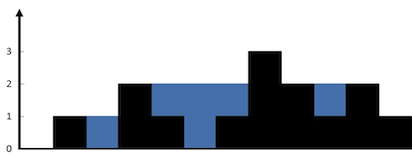
\includegraphics[width=100pt]{water.png}\\
\end{center}

\subsubsection{Analysis}
核心思路就是对于每根柱子,找到其左边最高的柱子和右边最高的柱子,构成一个桶,形成一个水平面,然后对该柱子形成的高度差就是能装的水

\subsubsection{Solution}

\begin{Code}
// 耗时24ms
public int trap(int[] height) {
    int len = height.length;

    if (len == 0) {
        return 0;
    }

    int[] left = new int[len];
    int[] right = new int[len];

    left[0] = 0;
    right[len - 1] = 0;

    for (int i = 1; i < len; i++) {
        left[i] = Math.max(left[i - 1], height[i - 1]);
    }
    for (int i = len - 2; i>= 0; i--) {
        right[i] = Math.max(right[i + 1], height[i + 1]);
    }
    int sum = 0;
    for (int i = 0; i < len; i++) {
        int high = Math.min(left[i], right[i]);
        if (high > height[i]) {
            sum += high - height[i];
        }
    }
    return sum;
}
\end{Code}

\newpage

\section{Trapping Rain Water II} %%%%%%%%%%%%%%%%%%%%%%



\subsubsection{Description}
Given an m x n matrix of positive integers representing the height of each unit cell in a 2D elevation map, compute the volume of water it is able to trap after raining.

\textbf{Note:}

Both m and n are less than 110. The height of each unit cell is greater than 0 and is less than 20,000.

\textbf{Example:}

Given the following 3x6 height map:
\begin{Code}
[
  [1,4,3,1,3,2],
  [3,2,1,3,2,4],
  [2,3,3,2,3,1]
]
\end{Code}
Return 4.

\begin{center}
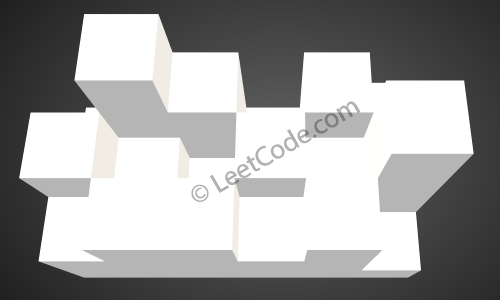
\includegraphics[width=150pt]{water2.png}\\
\end{center}

The above image represents the elevation map [[1,4,3,1,3,2],[3,2,1,3,2,4],[2,3,3,2,3,1]] before the rain.

\begin{center}
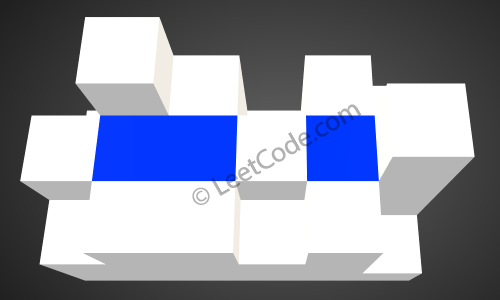
\includegraphics[width=150pt]{water3.png}\\
\end{center}

After the rain, water are trapped between the blocks. The total volume of water trapped is 4.

\subsubsection{Analysis}
思路是从外围开始,选择最短的柱子,以该柱子为标准,计算其四周的柱子所能容纳的水,并且更新四周柱子的高度,并加到小堆中。为什么这样呢?一个柱子所能蓄的水和该柱子相邻的四根柱子有关,所以我们从边界开始,不断向中间靠拢,每次都取队列中最短的那根柱子计算

\newpage

\subsubsection{Solution}

\begin{Code}
public int trapRainWater(int[][] heightMap) {
    if (heightMap.length == 0) {
        return 0;
    }
    Queue<int[]> queue = new PriorityQueue<>(new Comparator<int[]>() {
        @Override
        public int compare(int[] o1, int[] o2) {
            return o1[2] - o2[2];
        }
    });
    int row = heightMap.length, col = heightMap[0].length;
    boolean[][] visited = new boolean[row][col];
    for (int i = 0; i < col; i++) {
        queue.add(new int[] {0, i, heightMap[0][i]});
        queue.add(new int[] {row - 1, i, heightMap[row - 1][i]});
        visited[0][i] = true;
        visited[row - 1][i] = true;
    }
    for (int i = 0; i < row; i++) {
        queue.add(new int[] {i, 0, heightMap[i][0]});
        queue.add(new int[] {i, col - 1, heightMap[i][col - 1]});
        visited[i][0] = true;
        visited[i][col - 1] = true;
    }
    int res = 0;
    int[][] delta = new int[][] {
            {-1, 0}, {1, 0}, {0, -1}, {0, 1}
    };
    while (!queue.isEmpty()) {
        int[] node = queue.poll();
        int x = node[0], y = node[1], z = node[2];
        for (int i = 0; i < delta.length; i++) {
            int xx = x + delta[i][0], yy = y + delta[i][1];
            if (xx >= 0 && xx < row && yy >= 0 && yy < col && !visited[xx][yy]) {
                visited[xx][yy] = true;
                res += Math.max(0, z - heightMap[xx][yy]);
                /**
                 * 这里要更新柱子的高度,因为水平面肯定是Math.max(z, heightMap[xx][yy])
                 */
                queue.add(new int[] {xx, yy, Math.max(z, heightMap[xx][yy])});
            }
        }
    }
    return res;
}
\end{Code}

\newpage

\section{Product of Array Except Self} %%%%%%%%%%%%%%%%%%%%%%



\subsubsection{Description}
Given an array of n integers where n > 1, nums, return an array output such that output[i] is equal to the product of all the elements of nums except nums[i].

Solve it without division and in O(n).

For example, given [1,2,3,4], return [24,12,8,6].

\textbf{Follow up:}

Could you solve it with constant space complexity? (Note: The output array does not count as extra space for the purpose of space complexity analysis.)

\subsubsection{Solution}

\begin{Code}
public int[] productExceptSelf(int[] nums) {
    if (nums.length == 0) {
        return null;
    }
    int[] result = new int[nums.length];
    result[0] = 1;
    for (int i = 1; i < nums.length; i++) {
        result[i] = nums[i - 1] * result[i - 1];
    }
    int right = 1;
    for (int i = nums.length - 1; i >= 0; i--) {
        result[i] *= right;
        right *= nums[i];
    }
    return result;
}
\end{Code}

\newpage

\section{Find Minimum in Rotated Sorted Array} %%%%%%%%%%%%%%%%%%%%%%



\subsubsection{Description}
Suppose an array sorted in ascending order is rotated at some pivot unknown to you beforehand.

(i.e., 0 1 2 4 5 6 7 might become 4 5 6 7 0 1 2).

Find the minimum element.

You may assume no duplicate exists in the array.
\subsubsection{Solution}

\begin{Code}
public int findMin(int[] nums) {
    for (int left = 0, right = nums.length - 1; left >= 0 && left <= right; ) {
        if (nums[right] > nums[left]) {
            return nums[left];
        }
        int mid = left + ((right - left) >> 1);

        if (nums[mid] > nums[left]) {
            left = mid + 1;
        } else if (nums[mid] < nums[right]) {
            right = mid;
        } else {
            return Math.min(nums[left], nums[right]);
        }
    }
    return 0;
}
\end{Code}

\newpage

\section{Find Minimum in Rotated Sorted Array II} %%%%%%%%%%%%%%%%%%%%%%



\subsubsection{Description}
Follow up for "Find Minimum in Rotated Sorted Array":

What if duplicates are allowed?

Would this affect the run-time complexity? How and why?
Suppose an array sorted in ascending order is rotated at some pivot unknown to you beforehand.

(i.e., 0 1 2 4 5 6 7 might become 4 5 6 7 0 1 2).

Find the minimum element.

The array may contain duplicates.

\subsubsection{Solution}

\begin{Code}
public int findMin(int[] nums) {
    int left = 0, right = nums.length - 1;

    for ( ; left < right; ) {
        int mid = left + ((right - left) >> 1);

        if (nums[right] > nums[left]) {
            return nums[left];
        }

        if (nums[mid] > nums[left]) {
            left = mid + 1;
        } else if (nums[mid] < nums[right]) {
            right = mid;
        } else {
            left++;
        }
    }

    return nums[left];
}
\end{Code}

\newpage

\section{Search in Rotated Sorted Array} %%%%%%%%%%%%%%%%%%%%%%



\subsubsection{Description}
Suppose an array sorted in ascending order is rotated at some pivot unknown to you beforehand.

(i.e., 0 1 2 4 5 6 7 might become 4 5 6 7 0 1 2).

You are given a target value to search. If found in the array return its index, otherwise return -1.

You may assume no duplicate exists in the array.

\subsubsection{Solution}

\begin{Code}
public int search(int[] nums, int target) {
    int left = 0, right = nums.length - 1;

    // 注意这里的等号
    while (left <= right) {
        int mid = left + ((right - left) >>> 1);

        if (target == nums[mid]) {
            return mid;
        }

        // 注意这里的等号
        // 先确定单调区间,然后判断target是不是在单调区间内,如果不在就在另一半区间
        if (nums[mid] >= nums[left]) {
            if (target >= nums[left] && target < nums[mid]) {
                right = mid - 1;
            } else {
                left = mid + 1;
            }
        } else if (nums[mid] < nums[right]) {
            if (target > nums[mid] && target <= nums[right]) {
                left = mid + 1;
            } else {
                right = mid - 1;
            }
        }
    }

    return -1;
}
\end{Code}

\newpage

\section{Search in Rotated Sorted Array II} %%%%%%%%%%%%%%%%%%%%%%



\subsubsection{Description}
Follow up for "Search in Rotated Sorted Array":
What if duplicates are allowed?

Would this affect the run-time complexity? How and why?
Suppose an array sorted in ascending order is rotated at some pivot unknown to you beforehand.

(i.e., 0 1 2 4 5 6 7 might become 4 5 6 7 0 1 2).

Write a function to determine if a given target is in the array.

The array may contain duplicates.

\subsubsection{Solution}

\begin{Code}
public int search(int[] nums, int target) {
    int left = 0, right = nums.length - 1;

    // 注意这里的等号
    while (left <= right) {
        int mid = left + ((right - left) >>> 1);

        if (target == nums[mid]) {
            return mid;
        }

        // 注意这里的等号
        // 先确定单调区间,然后判断target是不是在单调区间内,如果不在就在另一半区间
        if (nums[mid] > nums[left]) {
            if (target >= nums[left] && target < nums[mid]) {
                right = mid - 1;
            } else {
                left = mid + 1;
            }
        } else if (nums[mid] == nums[left]) {
            // nums[mid]==nums[left]有两种情况,在不好确定哪种情况时,left++可以进一步缩小范围
            left++;
        } else {
            // 这里可以肯定nums[mid]<nums[left],所以mid肯定在拐点右边,换言之右边是单调的
            if (target > nums[mid] && target <= nums[right]) {
                left = mid + 1;
            } else {
                right = mid - 1;
            }
        }
    }

    return -1;
}
\end{Code}

\newpage

\section{Pascal's Triangle} %%%%%%%%%%%%%%%%%%%%%%



\subsubsection{Description}
Given numRows, generate the first numRows of Pascal's triangle.

For example, given numRows = 5,

Return
\begin{Code}
[
     [1],
    [1,1],
   [1,2,1],
  [1,3,3,1],
 [1,4,6,4,1]
]
\end{Code}
\subsubsection{Solution}

\begin{Code}
public List<List<Integer>> generate(int numRows) {
    List<List<Integer>> allrows = new ArrayList<>();
    ArrayList<Integer> row = new ArrayList<>();
    for (int i = 0; i < numRows; i++) {
        row.add(0, 1);
        for (int j = 1; j < row.size() - 1; j++)
            row.set(j, row.get(j) + row.get(j + 1));
        allrows.add(new ArrayList<>(row));
    }
    return allrows;

}
\end{Code}

\newpage

\section{Pascal's Triangle II} %%%%%%%%%%%%%%%%%%%%%%



\subsubsection{Description}
Given an index k, return the kth row of the Pascal's triangle.

For example, given k = 3,

Return [1,3,3,1].

\textbf{Note:}

Could you optimize your algorithm to use only O(k) extra space?

\subsubsection{Solution}

\begin{Code}
public List<Integer> getRow(int rowIndex) {
    List<Integer> list = new ArrayList<>();

    for (int i = 0; i <= rowIndex; i++) {
        int prev = 1;
        for (int j = 1; j < list.size(); j++) {
            int n = list.get(j) + prev;
            prev = list.get(j);
            list.set(j, n);
        }
        list.add(1);
    }

    return list;
}
\end{Code}

\newpage

\section{Remove Element} %%%%%%%%%%%%%%%%%%%%%%



\subsubsection{Description}
Given an array and a value, remove all instances of that value in place and return the new length.

Do not allocate extra space for another array, you must do this in place with constant memory.

The order of elements can be changed. It doesn't matter what you leave beyond the new length.

\textbf{Example:}

Given input array nums = [3,2,2,3], val = 3

Your function should return length = 2, with the first two elements of nums being 2.

\subsubsection{Solution}

\begin{Code}
public int removeElement(int[] nums, int val) {
    int index = 0;

    for (int i = 0; i < nums.length; i++) {
        if (nums[i] != val) {
            nums[index++] = nums[i];
        }
    }

    return index;
}
\end{Code}

\newpage

\section{Summary Ranges} %%%%%%%%%%%%%%%%%%%%%%



\subsubsection{Description}
Given a sorted integer array without duplicates, return the summary of its ranges.

\textbf{Example 1:}

\textbf{Input:} [0,1,2,4,5,7]

\textbf{Output:} ["0->2","4->5","7"]

\textbf{Example 2:}

\textbf{Input:} [0,2,3,4,6,8,9]

\textbf{Output:} ["0","2->4","6","8->9"]

\subsubsection{Solution}

\begin{Code}
public List<String> summaryRanges(int[] nums) {
    List<String> list = new ArrayList();
    if (nums.length == 1) {
        list.add(nums[0] + "");
        return list;
    }
    for (int i = 0; i < nums.length; i++) {
        int a = nums[i];
        while (i + 1 < nums.length && (nums[i + 1] - nums[i]) == 1) {
            i++;
        }
        if (a != nums[i]) {
            list.add(a + "->" + nums[i]);
        } else {
            list.add(a + "");
        }
    }
    return list;
}
\end{Code}

\newpage

\section{Merge Sorted Array} %%%%%%%%%%%%%%%%%%%%%%



\subsubsection{Description}
Given two sorted integer arrays nums1 and nums2, merge nums2 into nums1 as one sorted array.

\textbf{Note:}

You may assume that nums1 has enough space (size that is greater or equal to m + n) to hold additional elements from nums2. The number of elements initialized in nums1 and nums2 are m and n respectively.

\subsubsection{Solution}

\begin{Code}
public void merge(int[] nums1, int m, int[] nums2, int n) {
    int j = m - 1, k = n - 1;
    for (int i = m + n - 1; i >= 0; i--) {
        if (j < 0) {
            nums1[i] = nums2[k--];
        } else if (k < 0) {
            nums1[i] = nums1[j--];
        } else {
            if (nums1[j] >= nums2[k]) {
                nums1[i] = nums1[j--];
            } else {
                nums1[i] = nums2[k--];
            }
        }
    }
}
\end{Code}

\newpage

\section{Rotate Image} %%%%%%%%%%%%%%%%%%%%%%



\subsubsection{Description}
You are given an n x n 2D matrix representing an image.

Rotate the image by 90 degrees (clockwise).

\textbf{Note:}

You have to rotate the image in-place, which means you have to modify the input 2D matrix directly. DO NOT allocate another 2D matrix and do the rotation.

\textbf{Example 1:}

Given input matrix =
\begin{Code}
[
  [1,2,3],
  [4,5,6],
  [7,8,9]
],
\end{Code}

rotate the input matrix in-place such that it becomes:
\begin{Code}
[
  [7,4,1],
  [8,5,2],
  [9,6,3]
]
\end{Code}

\subsubsection{Solution}

\begin{Code}
// 耗时2ms
public void rotate(int[][] matrix) {
    int n = matrix.length;

    for (int i = 0; i < n / 2; i++) {
        for (int j = 0; j < n; j++) {
            int t = matrix[i][j];
            matrix[i][j] = matrix[n - 1 - i][j];
            matrix[n - 1 - i][j] = t;
        }
    }

    for (int i = 0; i < n; i++) {
        for (int j = 0; j < i; j++) {
            int t = matrix[i][j];
            matrix[i][j] = matrix[j][i];
            matrix[j][i] = t;
        }
    }
}
\end{Code}

\newpage

\section{Remove Duplicates from Sorted Array} %%%%%%%%%%%%%%%%%%%%%%



\subsubsection{Description}
Given a sorted array, remove the duplicates in place such that each element appear only once and return the new length.

Do not allocate extra space for another array, you must do this in place with constant memory.

For example,

Given input array nums = [1,1,2],

Your function should return length = 2, with the first two elements of nums being 1 and 2 respectively. It doesn't matter what you leave beyond the new length.

\subsubsection{Solution}

\begin{Code}
public int removeDuplicates(int[] nums) {
    int j = -1;
    for (int i = 0; i < nums.length; i++) {
        if (j == -1 || nums[i] != nums[j]) {
            nums[++j] = nums[i];
        }
    }
    return j + 1;
}
\end{Code}

\newpage

\section{Remove Duplicates from Sorted Array II} %%%%%%%%%%%%%%%%%%%%%%



\subsubsection{Description}
Follow up for "Remove Duplicates":
What if duplicates are allowed at most twice?

For example,
Given sorted array nums = [1,1,1,2,2,3],

Your function should return length = 5, with the first five elements of nums being 1, 1, 2, 2 and 3. It doesn't matter what you leave beyond the new length.

\subsubsection{Solution}

\begin{Code}
public int removeDuplicates(int[] nums) {
    int j = -1;
    for (int i = 0; i < nums.length; i++) {
        if (j < 1 || nums[i] != nums[j - 1]) {
            nums[++j] = nums[i];
        }
    }
    return j + 1;
}
\end{Code}

\newpage

\section{Rotate Array} %%%%%%%%%%%%%%%%%%%%%%



\subsubsection{Description}
Rotate an array of n elements to the right by k steps.

For example, with n = 7 and k = 3, the array [1,2,3,4,5,6,7] is rotated to [5,6,7,1,2,3,4].

\textbf{Note:}

Try to come up as many solutions as you can, there are at least 3 different ways to solve this problem.

\textbf{Hint:}

Could you do it in-place with O(1) extra space?

\subsubsection{Solution}

\begin{Code}
public void rotate(int[] nums, int k) {
    k %= nums.length;
    reverse(nums, 0, nums.length - 1);
    reverse(nums, 0, k - 1);
    reverse(nums, k, nums.length - 1);
}

public void reverse(int[] nums, int start, int end) {
    while (start < end) {
        int temp = nums[start];
        nums[start] = nums[end];
        nums[end] = temp;
        start++;
        end--;
    }
}
\end{Code}

\newpage

\section{Spiral Matrix} %%%%%%%%%%%%%%%%%%%%%%



\subsubsection{Description}
Given a matrix of m x n elements (m rows, n columns), return all elements of the matrix in spiral order.

For example,

Given the following matrix:
\begin{Code}
[
 [ 1, 2, 3 ],
 [ 4, 5, 6 ],
 [ 7, 8, 9 ]
]
\end{Code}

You should return [1,2,3,6,9,8,7,4,5].


\subsubsection{Solution}

\begin{Code}
public List<Integer> spiralOrder(int[][] matrix) {
    List<Integer> res = new ArrayList<Integer>();
    if (matrix.length == 0) { return res; }

    int rowBegin = 0, rowEnd = matrix.length - 1;
    int colBegin = 0, colEnd = matrix[0].length - 1;

    while (rowBegin <= rowEnd && colBegin <= colEnd) {
        for (int j = colBegin; j <= colEnd; j++) {
            res.add(matrix[rowBegin][j]);
        }
        rowBegin++;

        for (int j = rowBegin; j <= rowEnd; j++) {
            res.add(matrix[j][colEnd]);
        }
        colEnd--;

        if (rowBegin <= rowEnd) {
            for (int j = colEnd; j >= colBegin; j--) {
                res.add(matrix[rowEnd][j]);
            }
        }
        rowEnd--;

        if (colBegin <= colEnd) {
            for (int j = rowEnd; j >= rowBegin; j--) {
                res.add(matrix[j][colBegin]);
            }
        }
        colBegin++;
    }

    return res;
}
\end{Code}

\newpage

\section{Merge Intervals} %%%%%%%%%%%%%%%%%%%%%%



\subsubsection{Description}
Given a collection of intervals, merge all overlapping intervals.

For example,

Given [1,3],[2,6],[8,10],[15,18],

return [1,6],[8,10],[15,18].

\subsubsection{Solution}

\begin{Code}
// 耗时26ms,时间复杂度O(nlgn)
public List<Interval> merge(List<Interval> intervals) {
    List<Interval> result = new LinkedList<Interval>();
    if (intervals.size() == 0) {
        return result;
    }
    Collections.sort(intervals, new Comparator<Interval>() {
        @Override
        public int compare(Interval o1, Interval o2) {
            return o1.start - o2.start;
        }
    });
    Interval prev = null;
    for (Interval interval : intervals) {
        if (prev == null) {
            prev = interval;
        } else {
            if (interval.start > prev.end) {
                result.add(prev);
                prev = interval;
            } else {
                prev.end = Math.max(prev.end, interval.end);
            }
        }
    }
    result.add(prev);
    return result;
}
\end{Code}

\newpage

\section{Insert Interval} %%%%%%%%%%%%%%%%%%%%%%



\subsubsection{Description}
Given a set of non-overlapping intervals, insert a new interval into the intervals (merge if necessary).

You may assume that the intervals were initially sorted according to their start times.

\textbf{Example 1:}

Given intervals [1,3],[6,9], insert and merge [2,5] in as [1,5],[6,9].

\textbf{Example 2:}

Given [1,2],[3,5],[6,7],[8,10],[12,16], insert and merge [4,9] in as [1,2],[3,10],[12,16].

This is because the new interval [4,9] overlaps with [3,5],[6,7],[8,10].

\subsubsection{Solution}

\begin{Code}
public List<Interval> insert(List<Interval> intervals, Interval newInterval) {
    List<Interval> result = new LinkedList<Interval>();
    for (Interval interval : intervals) {
        if (newInterval.start > interval.end) {
            result.add(interval);
        } else if (newInterval.end < interval.start) {
            result.add(newInterval);
            newInterval = interval;
        } else {
            newInterval.start = Math.min(interval.start, newInterval.start);
            newInterval.end = Math.max(interval.end, newInterval.end);
        }
    }
    result.add(newInterval);
    return result;
}
\end{Code}

\newpage

\section{Meeting Rooms} %%%%%%%%%%%%%%%%%%%%%%



\subsubsection{Description}
Given an array of meeting time intervals consisting of start and end times [[s1,e1],[s2,e2],...] (si < ei), determine if a person could attend all meetings.

For example,

Given [[0, 30],[5, 10],[15, 20]],

return false.

\subsubsection{Solution}

\begin{Code}
// 时间复杂度O(nlgn)
public boolean canAttendMeetings(Interval[] intervals) {
    Arrays.sort(intervals, new Comparator<Interval>() {
        @Override
        public int compare(Interval o1, Interval o2) {
            return o1.start > o2.start ? 1 : -1;
        }
    });

    for (int i = 1; i < intervals.length; i++) {
        if (intervals[i].start < intervals[i - 1].end) {
            return false;
        }
    }

    return true;
}
\end{Code}

\newpage

\section{Meeting Rooms II} %%%%%%%%%%%%%%%%%%%%%%



\subsubsection{Description}
Given an array of meeting time intervals consisting of start and end times [[s1,e1],[s2,e2],...] (si < ei), find the minimum number of conference rooms required.

For example,

Given [[0, 30],[5, 10],[15, 20]],

return 2.

\subsubsection{Solution}

\begin{Code}
// 耗时17ms,时间复杂度O(nlgn)
public int minMeetingRooms(Interval[] intervals) {
    Arrays.sort(intervals, new Comparator<Interval>() {
        @Override
        public int compare(Interval o1, Interval o2) {
            return o1.start - o2.start;
        }
    });
    Queue<Interval> queue = new PriorityQueue<Interval>(new Comparator<Interval>() {
        @Override
        public int compare(Interval o1, Interval o2) {
            return o1.end - o2.end;
        }
    });
    for (Interval interval : intervals) {
        if (!queue.isEmpty() && interval.start >= queue.peek().end) {
            queue.poll();
        }
        queue.add(interval);
    }
    return queue.size();
}
\end{Code}

\newpage

\section{Find the Duplicate Number} %%%%%%%%%%%%%%%%%%%%%%



\subsubsection{Description}
Given an array nums containing n + 1 integers where each integer is between 1 and n (inclusive), prove that at least one duplicate number must exist. Assume that there is only one duplicate number, find the duplicate one.

\textbf{Note:}

1. You must not modify the array (assume the array is read only).

2. You must use only constant, O(1) extra space.

3. Your runtime complexity should be less than O(n2).

4. There is only one duplicate number in the array, but it could be repeated more than once.

\subsubsection{Solution}

\begin{Code}
public int findDuplicate(int[] nums) {
    int min = 1, max = nums.length - 1;

    while (min < max) {
        int mid = (min + max) / 2;

        int count = 0;

        for (int i = 0; i < nums.length; i++) {
            if (nums[i] <= mid) {
                count++;
            }
        }

        if (count > mid) {
            max = mid;
        } else {
            min = mid + 1;
        }
    }

    return min;
}
\end{Code}

\newpage

\section{Missing Number} %%%%%%%%%%%%%%%%%%%%%%



\subsubsection{Description}
Given an array containing n distinct numbers taken from 0, 1, 2, ..., n, find the one that is missing from the array.

For example,

Given nums = [0, 1, 3] return 2.

\textbf{Note:}

Your algorithm should run in linear runtime complexity. Could you implement it using only constant extra space complexity?
\subsubsection{Solution}

\begin{Code}
public int missingNumber(int[] nums) {
    int xor = 0, i = 0;
    for (i = 0; i < nums.length; i++) {
        xor = xor ^ i ^ nums[i];
    }

    return xor ^ i;
}
\end{Code}

\newpage

\section{Find Peak Element} %%%%%%%%%%%%%%%%%%%%%%



\subsubsection{Description}
A peak element is an element that is greater than its neighbors.

Given an input array where num[i] ≠ num[i+1], find a peak element and return its index.

The array may contain multiple peaks, in that case return the index to any one of the peaks is fine.

You may imagine that num[-1] = num[n] = -∞.

For example, in array [1, 2, 3, 1], 3 is a peak element and your function should return the index number 2.

\textbf{Note:}

Your solution should be in logarithmic complexity.
\subsubsection{Solution}

\begin{Code}
public int findPeakElement(int[] nums) {
    return Helper(nums, 0, nums.length - 1);
}

private int Helper(int[] nums, int low, int high) {
    if (low == high) {
        return low;
    } else {
        int mid1 = (low + high) / 2;
        int mid2 = mid1 + 1;
        if (nums[mid1] > nums[mid2]) {
            return Helper(nums, low, mid1);
        } else {
            return Helper(nums, mid2, high);
        }
    }
}
\end{Code}

\newpage

\section{Majority Element} %%%%%%%%%%%%%%%%%%%%%%



\subsubsection{Description}
Given an array of size n, find the majority element. The majority element is the element that appears more than ⌊ n/2 ⌋ times.

You may assume that the array is non-empty and the majority element always exist in the array.

\subsubsection{Solution}

\begin{Code}
public int majorityElement(int[] nums) {
    int major = nums[0], count = 1;
    for (int i = 1; i < nums.length; i++) {
        if (count == 0) {
            count++;
            major = nums[i];
        } else if (major == nums[i]) {
            count++;
        } else {
            count--;
        }
    }
    return major;
}
\end{Code}

\newpage

\section{Majority Element II} %%%%%%%%%%%%%%%%%%%%%%



\subsubsection{Description}
Given an integer array of size n, find all elements that appear more than ⌊ n/3 ⌋ times. The algorithm should run in linear time and in O(1) space.

\subsubsection{Solution}

\begin{Code}
public List<Integer> majorityElement(int[] nums) {
    if (nums == null || nums.length == 0)
        return new ArrayList<Integer>();
    List<Integer> result = new ArrayList<Integer>();
    int number1 = nums[0], number2 = nums[0], count1 = 0, count2 = 0, len = nums.length;
    for (int i = 0; i < len; i++) {
        if (nums[i] == number1)
            count1++;
        else if (nums[i] == number2)
            count2++;
        else if (count1 == 0) {
            number1 = nums[i];
            count1 = 1;
        } else if (count2 == 0) {
            number2 = nums[i];
            count2 = 1;
        } else {
            count1--;
            count2--;
        }
    }
    count1 = 0;
    count2 = 0;
    for (int i = 0; i < len; i++) {
        if (nums[i] == number1)
            count1++;
        else if (nums[i] == number2)
            count2++;
    }
    if (count1 > len / 3)
        result.add(number1);
    if (count2 > len / 3)
        result.add(number2);
    return result;
}
\end{Code}

\newpage

\section{First Missing Positive} %%%%%%%%%%%%%%%%%%%%%%



\subsubsection{Description}
Given an unsorted integer array, find the first missing positive integer.

For example,

Given [1,2,0] return 3,

and [3,4,-1,1] return 2.

Your algorithm should run in O(n) time and uses constant space.

\subsubsection{Analysis}
 这里要注意的是nums[nums[i] - 1] != nums[i]这个条件,意思是目标坑和当前坑的值不等,此时才能swap
 倘若换成nums[i] - 1 != i是不行的,这表示目标坑和当前坑不是一个坑就swap,会死循环

\subsubsection{Solution}

\begin{Code}
public int firstMissingPositive(int[] nums) {
    for (int i = 0; i < nums.length; i++) {
        while (nums[i] >= 1 && nums[i] <= nums.length && nums[nums[i] - 1] != nums[i]) {
            swap(nums, i, nums[i] - 1);
        }
    }
    for (int i = 0; i < nums.length; i++) {
        if (i != nums[i] - 1) {
            return i + 1;
        }
    }
    return nums.length + 1;
}

private void swap(int[] nums, int i, int j) {
    if (i != j) {
        int t = nums[i];
        nums[i] = nums[j];
        nums[j] = t;
    }
}
\end{Code}

\newpage

\section{Game of Life} %%%%%%%%%%%%%%%%%%%%%%



\subsubsection{Description}
According to the Wikipedia's article: "The Game of Life, also known simply as Life, is a cellular automaton devised by the British mathematician John Horton Conway in 1970."

Given a board with m by n cells, each cell has an initial state live (1) or dead (0). Each cell interacts with its eight neighbors (horizontal, vertical, diagonal) using the following four rules (taken from the above Wikipedia article):

1. Any live cell with fewer than two live neighbors dies, as if caused by under-population.

2. Any live cell with two or three live neighbors lives on to the next generation.

3. Any live cell with more than three live neighbors dies, as if by over-population..

4. Any dead cell with exactly three live neighbors becomes a live cell, as if by reproduction.

Write a function to compute the next state (after one update) of the board given its current state.

\textbf{Follow up:}

1. Could you solve it in-place? Remember that the board needs to be updated at the same time: You cannot update some cells first and then use their updated values to update other cells.

2. In this question, we represent the board using a 2D array. In principle, the board is infinite, which would cause problems when the active area encroaches the border of the array. How would you address these problems?

\newpage

\subsubsection{Solution}

\begin{Code}
public void gameOfLife(int[][] board) {
    if (board == null || board.length == 0) return;
    int m = board.length, n = board[0].length;

    for (int i = 0; i < m; i++) {
        for (int j = 0; j < n; j++) {
            int lives = liveNeighbors(board, m, n, i, j);

            // In the beginning, every 2nd bit is 0;
            // So we only need to care about when will the 2nd bit become 1.
            if (board[i][j] == 1 && lives >= 2 && lives <= 3) {
                board[i][j] = 3; // Make the 2nd bit 1: 01 ---> 11
            }
            if (board[i][j] == 0 && lives == 3) {
                board[i][j] = 2; // Make the 2nd bit 1: 00 ---> 10
            }
        }
    }

    for (int i = 0; i < m; i++) {
        for (int j = 0; j < n; j++) {
            board[i][j] >>= 1;  // Get the 2nd state.
        }
    }
}

public int liveNeighbors(int[][] board, int m, int n, int i, int j) {
    int lives = 0;
    for (int x = Math.max(i - 1, 0); x <= Math.min(i + 1, m - 1); x++) {
        for (int y = Math.max(j - 1, 0); y <= Math.min(j + 1, n - 1); y++) {
            lives += board[x][y] & 1;
        }
    }
    lives -= board[i][j] & 1;
    return lives;
}
\end{Code}

\newpage

\section{Set Matrix Zeroes} %%%%%%%%%%%%%%%%%%%%%%



\subsubsection{Description}
Given a m x n matrix, if an element is 0, set its entire row and column to 0. Do it in place.

\textbf{Follow up:}

Did you use extra space?

A straight forward solution using O(mn) space is probably a bad idea.

A simple improvement uses O(m + n) space, but still not the best solution.

Could you devise a constant space solution?

\newpage

\subsubsection{Solution}

\begin{Code}
public void setZeroes(int[][] matrix) {
    if (matrix.length == 0) {
        return;
    }
    int row = matrix.length, col = matrix[0].length;
    boolean clearRow = false, clearCol = false;

    for (int i = 0; i < col; i++) {
        if (matrix[0][i] == 0) {
            clearRow = true;
            break;
        }
    }
    for (int i = 0; i < row; i++) {
        if (matrix[i][0] == 0) {
            clearCol = true;
            break;
        }
    }
    for (int i = 1; i < row; i++) {
        for (int j = 1; j < col; j++) {
            if (matrix[i][j] == 0) {
                matrix[0][j] = 0;
                matrix[i][0] = 0;
            }
        }
    }

    for (int i = 1; i < col; i++) {
        if (matrix[0][i] == 0) {
            for (int j = 0; j < row; j++) {
                matrix[j][i] = 0;
            }
        }
    }

    for (int i = 1; i < row; i++) {
        if (matrix[i][0] == 0) {
            for (int j = 0; j < col; j++) {
                matrix[i][j] = 0;
            }
        }
    }

    if (clearRow) {
        for (int i = 0; i < col; i++) {
            matrix[0][i] = 0;
        }
    }

    if (clearCol) {
        for (int i = 0; i < row; i++) {
            matrix[i][0] = 0;
        }
    }
}
\end{Code}

\newpage

\section{Next Permutation} %%%%%%%%%%%%%%%%%%%%%%



\subsubsection{Description}
Implement next permutation, which rearranges numbers into the lexicographically next greater permutation of numbers.

If such arrangement is not possible, it must rearrange it as the lowest possible order (ie, sorted in ascending order).

The replacement must be in-place, do not allocate extra memory.

Here are some examples. Inputs are in the left-hand column and its corresponding outputs are in the right-hand column.
\begin{Code}
1,2,3 → 1,3,2
3,2,1 → 1,2,3
1,1,5 → 1,5,1
\end{Code}

\subsubsection{Solution}

\begin{Code}
public void nextPermutation(int[] nums) {
    int i = nums.length - 1;

    for ( ; i >= 0; i--) {
        if (i > 0 && nums[i - 1] < nums[i]) {
            break;
        }
    }

    if (i < 0) {
        revert(nums, 0, nums.length - 1);
        return;
    }

    int index = searchSwapPoint(nums, i, nums.length - 1, nums[i - 1]);

    swap(nums, i - 1, index);
    revert(nums, i, nums.length - 1);
}
\end{Code}

\newpage

\begin{Code}
private int searchSwapPoint(int[] nums, int left, int right, int target) {
    while (left <= right) {
        int mid = left + ((right - left) >> 1);

        if (left == mid) {
            if (target >= nums[right]) {
                return right - 1;
            } else {
                return right;
            }
        }

        if (target > nums[mid]) {
            right = mid - 1;
        } else if (target < nums[mid]) {
            left = mid;
        } else {
            right = mid - 1;
        }
    }

    throw new IllegalStateException("");
}

private void swap(int[] nums, int left, int right) {
    int temp = nums[left];
    nums[left] = nums[right];
    nums[right] = temp;
}

private void revert(int[] nums, int start, int end) {
    for ( ; start < end; start++, end--) {
        swap(nums, start, end);
    }
}
\end{Code}

\newpage

\section{Search for a Range} %%%%%%%%%%%%%%%%%%%%%%



\subsubsection{Description}
Given an array of integers sorted in ascending order, find the starting and ending position of a given target value.

Your algorithm's runtime complexity must be in the order of O(log n).

If the target is not found in the array, return [-1, -1].

For example,

Given [5, 7, 7, 8, 8, 10] and target value 8,

return [3, 4].

\subsubsection{Solution}

\begin{Code}
public int[] searchRange(int[] nums, int target) {
    int len = nums.length;

    int left, right;

    int[] result = new int[] { -1, -1 };

    for (left = 0, right = len - 1; left < right; ) {
        int mid = (left + right) / 2;

        if (target > nums[mid]) {
            left = mid + 1;
        } else {
            right = mid;
        }
    }

    if (nums[left] != target) {
        return result;
    } else {
        result[0] = left;
    }

    for (right = len - 1; left < right; ) {
        int mid = (left + right) / 2 + 1;

        if (target < nums[mid]) {
            right = mid - 1;
        } else {
            left = mid;
        }
    }

    result[1] = right;

    return result;
}
\end{Code}

\newpage

\section{Search a 2D Matrix} %%%%%%%%%%%%%%%%%%%%%%



\subsubsection{Description}
Write an efficient algorithm that searches for a value in an m x n matrix. This matrix has the following properties:

Integers in each row are sorted from left to right.
The first integer of each row is greater than the last integer of the previous row.
For example,

Consider the following matrix:
\begin{Code}
[
  [1,   3,  5,  7],
  [10, 11, 16, 20],
  [23, 30, 34, 50]
]
\end{Code}

Given target = 3, return true.
\subsubsection{Solution}

\begin{Code}
// 耗时14ms
public boolean searchMatrix(int[][] matrix, int target) {
    int row = matrix.length;
    int col = matrix[0].length;

    int left = 0, right = row - 1;

    while (left < right) {
        int mid = (left + right) / 2 + 1;

        int n = matrix[mid][0];

        if (target == n) {
            return true;
        } else if (target < n) {
            right = mid - 1;
        } else {
            left = mid;
        }
    }

    if (target < matrix[right][0]) {
        return false;
    } else if (target == matrix[right][0]) {
        return true;
    }

    return Arrays.binarySearch(matrix[right], 0, col, target) >= 0;
}
\end{Code}

\newpage

\section{Search a 2D Matrix II} %%%%%%%%%%%%%%%%%%%%%%



\subsubsection{Description}
Write an efficient algorithm that searches for a value in an m x n matrix. This matrix has the following properties:

Integers in each row are sorted in ascending from left to right.
Integers in each column are sorted in ascending from top to bottom.
For example,

Consider the following matrix:
\begin{Code}
[
  [1,   4,  7, 11, 15],
  [2,   5,  8, 12, 19],
  [3,   6,  9, 16, 22],
  [10, 13, 14, 17, 24],
  [18, 21, 23, 26, 30]
]
\end{Code}

Given target = 5, return true.

Given target = 20, return false.

\subsubsection{Solution}

\begin{Code}
// 耗时14ms
public boolean searchMatrix(int[][] matrix, int target) {
    if (matrix.length == 0) {
        return false;
    }

    int row = matrix.length, col = matrix[0].length;

    for (int i = 0, j = col - 1; i < row && j >= 0; ) {
        if (target > matrix[i][j]) {
            i++;
        } else if (target < matrix[i][j]) {
            j--;
        } else {
            return true;
        }
    }

    return false;
}
\end{Code}

\newpage

\section{Search Insert Position} %%%%%%%%%%%%%%%%%%%%%%



\subsubsection{Description}
Given a sorted array and a target value, return the index if the target is found. If not, return the index where it would be if it were inserted in order.

You may assume no duplicates in the array.

Here are few examples.
\begin{Code}
[1,3,5,6], 5 → 2
[1,3,5,6], 2 → 1
[1,3,5,6], 7 → 4
[1,3,5,6], 0 → 0
\end{Code}

\subsubsection{Solution I}

\begin{Code}
public int searchInsert(int[] nums, int target) {
    int left = 0, right = nums.length - 1;

    while (left <= right) {
        int mid = (left + right) / 2;

        if (target == nums[mid]) {
            return mid;
        } else if (target > nums[mid]) {
            left = mid + 1;
        } else {
            right = mid - 1;
        }
    }

    return left;
}
\end{Code}

\subsubsection{Solution II}
\begin{Code}
public int searchInsert2(int[] nums, int target) {
    int index = Arrays.binarySearch(nums, 0, nums.length, target);
    return index >= 0 ? index : -(index + 1);
}
\end{Code}

\newpage

\section{Minimum Size Subarray Sum} %%%%%%%%%%%%%%%%%%%%%%



\subsubsection{Description}
Given an array of n positive integers and a positive integer s, find the minimal length of a contiguous subarray of which the sum ≥ s. If there isn't one, return 0 instead.

For example, given the array [2,3,1,2,4,3] and s = 7,

the subarray [4,3] has the minimal length under the problem constraint.

More practice:

If you have figured out the O(n) solution, try coding another solution of which the time complexity is O(n log n).
\subsubsection{Solution}

\begin{Code}
public int minSubArrayLen(int s, int[] nums) {
    int sum = 0, min = Integer.MAX_VALUE;
    for (int i = 0, j = 0; i < nums.length; i++) {
        sum += nums[i];
        /**
         * 这里别掉了等号
         */
        if (sum >= s) {
            for ( ; j < i; j++) {
                if (sum - nums[j] < s) {
                    break;
                }
                sum -= nums[j];
            }
            min = Math.min(min, i - j + 1);
        }
    }
    return min == Integer.MAX_VALUE ? 0 : min;
}
\end{Code}

\newpage

\section{Maximum Size Subarray Sum Equals k} %%%%%%%%%%%%%%%%%%%%%%



\subsubsection{Description}
Given an array nums and a target value k, find the maximum length of a subarray that sums to k. If there isn't one, return 0 instead.

\textbf{Note:}
The sum of the entire nums array is guaranteed to fit within the 32-bit signed integer range.

\textbf{Example 1:}

Given nums = [1, -1, 5, -2, 3], k = 3,

return 4. (because the subarray [1, -1, 5, -2] sums to 3 and is the longest)

\textbf{Example 2:}

Given nums = [-2, -1, 2, 1], k = 1,

return 2. (because the subarray [-1, 2] sums to 1 and is the longest)

\textbf{Follow Up:}

Can you do it in O(n) time?

\subsubsection{Solution}

\begin{Code}
// 耗时29ms,时间复杂度O(n)
public int maxSubArrayLen2(int[] nums, int k) {
    HashMap<Integer, Integer> map = new HashMap<>();
    int maxLen = 0;

    map.put(0, -1);

    for (int i = 0, sum = 0; i < nums.length; i++) {
        sum += nums[i];
        if (!map.containsKey(sum)) {
            map.put(sum, i);
        }

        int idx = map.getOrDefault(sum - k, -2);
        if (idx >= -1 && i - idx > maxLen) {
            maxLen = i - idx;
        }
    }

    return maxLen;
}
\end{Code}

\newpage

\section{Find the Celebrity} %%%%%%%%%%%%%%%%%%%%%%



\subsubsection{Description}
Suppose you are at a party with n people (labeled from 0 to n - 1) and among them, there may exist one celebrity. The definition of a celebrity is that all the other n - 1 people know him/her but he/she does not know any of them.

Now you want to find out who the celebrity is or verify that there is not one. The only thing you are allowed to do is to ask questions like: "Hi, A. Do you know B?" to get information of whether A knows B. You need to find out the celebrity (or verify there is not one) by asking as few questions as possible (in the asymptotic sense).

You are given a helper function bool knows(a, b) which tells you whether A knows B. Implement a function int findCelebrity(n), your function should minimize the number of calls to knows.

\textbf{Note:} There will be exactly one celebrity if he/she is in the party. Return the celebrity's label if there is a celebrity in the party. If there is no celebrity, return -1.

\subsubsection{Solution}

\begin{Code}
public int findCelebrity(int n) {
    int id = 0;
    for (int i = 1; i < n; i++) {
        if (knows(id, i)) {
            id = i;
        }
    }
    for (int i = 0; i < n; i++) {
        if (i == id) {
            continue;
        }
        if (knows(id, i) || !knows(i, id)) {
            return -1;
        }
    }
    return id;
}
\end{Code}

\newpage

\section{Find All Numbers Disappeared in an Array} %%%%%%%%%%%%%%%%%%%%%%



\subsubsection{Description}
Given an array of integers where 1 ≤ a[i] ≤ n (n = size of array), some elements appear twice and others appear once.

Find all the elements of [1, n] inclusive that do not appear in this array.

Could you do it without extra space and in O(n) runtime? You may assume the returned list does not count as extra space.

\textbf{Example:}

\textbf{Input:}

[4,3,2,7,8,2,3,1]

\textbf{Output:}

[5,6]

\subsubsection{Solution}

\begin{Code}
public List<Integer> findDisappearedNumbers(int[] nums) {
    List<Integer> ret = new ArrayList<Integer>();

    for(int i = 0; i < nums.length; i++) {
        int val = Math.abs(nums[i]) - 1;
        if(nums[val] > 0) {
            nums[val] = -nums[val];
        }
    }

    for(int i = 0; i < nums.length; i++) {
        if(nums[i] > 0) {
            ret.add(i+1);
        }
    }
    return ret;
}
\end{Code}

\newpage

\section{Shortest Word Distance} %%%%%%%%%%%%%%%%%%%%%%



\subsubsection{Description}
Given a list of words and two words word1 and word2, return the shortest distance between these two words in the list.

For example,

Assume that words = \code{["practice", "makes", "perfect", "coding", "makes"]}.

Given word1 = \code{“coding”}, word2 = \code{“practice”}, return 3.

Given word1 = \code{"makes"}, word2 = \code{"coding"}, return 1.

\textbf{Note:}

You may assume that word1 does not equal to word2, and word1 and word2 are both in the list.

\subsubsection{Solution}

\begin{Code}
// 耗时3ms
public int shortestDistance(String[] words, String word1, String word2) {
    List<Integer> indexs1 = new LinkedList<Integer>();
    List<Integer> indexs2 = new LinkedList<Integer>();
    for (int i = 0; i < words.length; i++) {
        if (words[i].equals(word1)) {
            indexs1.add(i);
        } else if (words[i].equals(word2)) {
            indexs2.add(i);
        }
    }

    int size1 = indexs1.size(), size2 = indexs2.size();
    int min = Math.abs(indexs1.get(size1 - 1) - indexs2.get(size2 - 1));
    for (int i = 0, j = 0; i < size1 && j < size2; ) {
        int index1 = indexs1.get(i);
        int index2 = indexs2.get(j);

        min = Math.min(min, Math.abs(index1 - index2));

        if (index1 < index2) {
            i++;
        } else if (index1 > index2) {
            j++;
        } else {
            return 0;
        }
    }

    return min;
}
\end{Code}

\newpage

\section{Shortest Word Distance II} %%%%%%%%%%%%%%%%%%%%%%



\subsubsection{Description}
This is a follow up of Shortest Word Distance. The only difference is now you are given the list of words and your method will be called repeatedly many times with different parameters. How would you optimize it?

Design a class which receives a list of words in the constructor, and implements a method that takes two words word1 and word2 and return the shortest distance between these two words in the list.

For example,
Assume that words = \code{["practice", "makes", "perfect", "coding", "makes"]}.

Given word1 = \code{“coding”}, word2 = \code{“practice”}, return 3.

Given word1 = \code{"makes"}, word2 = \code{"coding"}, return 1.

\textbf{Note:}

You may assume that word1 does not equal to word2, and word1 and word2 are both in the list.

\subsubsection{Solution}

\begin{Code}
public class ShortestWordDistanceII {

    private Map<String, List<Integer>> map;

    public ShortestWordDistanceII(String[] words) {
        map = new HashMap<String, List<Integer>>();
        for (int i = 0; i < words.length; i++) {
            String w = words[i];
            if (map.containsKey(w)) {
                map.get(w).add(i);
            } else {
                List<Integer> list = new ArrayList<Integer>();
                list.add(i);
                map.put(w, list);
            }
        }
    }

    public int shortest(String word1, String word2) {
        List<Integer> list1 = map.get(word1);
        List<Integer> list2 = map.get(word2);
        int ret = Integer.MAX_VALUE;
        for (int i = 0, j = 0; i < list1.size() && j < list2.size(); ) {
            int index1 = list1.get(i), index2 = list2.get(j);
            if (index1 < index2) {
                ret = Math.min(ret, index2 - index1);
                i++;
            } else {
                ret = Math.min(ret, index1 - index2);
                j++;
            }
        }
        return ret;
    }
}
\end{Code}

\newpage

\section{ Shortest Word Distance III} %%%%%%%%%%%%%%%%%%%%%%



\subsubsection{Description}
This is a follow up of Shortest Word Distance. The only difference is now word1 could be the same as word2.

Given a list of words and two words word1 and word2, return the shortest distance between these two words in the list.

word1 and word2 may be the same and they represent two individual words in the list.

For example,

Assume that words = \code{["practice", "makes", "perfect", "coding", "makes"]}.

Given word1 = \code{“makes”}, word2 = \code{“coding”}, return 1.

Given word1 = \code{"makes"}, word2 = \code{"makes"}, return 3.

\code{Note:}

You may assume word1 and word2 are both in the list.
\subsubsection{Solution}

\begin{Code}
public int shortestWordDistance(String[] words, String word1, String word2) {
    long dist = Integer.MAX_VALUE, i1 = dist, i2 = -dist;
    for (int i = 0; i < words.length; i++) {
        if (words[i].equals(word1))
            i1 = i;
        if (words[i].equals(word2)) {
            if (word1.equals(word2))
                i1 = i2;
            i2 = i;
        }
        dist = Math.min(dist, Math.abs(i1 - i2));
    }
    return (int) dist;
}
\end{Code}

\newpage

\section{Find All Duplicates in an Array} %%%%%%%%%%%%%%%%%%%%%%



\subsubsection{Description}
Given an array of integers, 1 ≤ a[i] ≤ n (n = size of array), some elements appear twice and others appear once.

Find all the elements that appear twice in this array.

Could you do it without extra space and in O(n) runtime?
\subsubsection{Solution}

\begin{Code}
public List<Integer> findDuplicates(int[] nums) {
    List<Integer> res = new ArrayList<>();
    for (int i = 0; i < nums.length; ++i) {
        int index = Math.abs(nums[i]) - 1;
        if (nums[index] < 0)
            res.add(Math.abs(index + 1));
        nums[index] = -nums[index];
    }
    return res;
}
\end{Code}

\newpage

\section{Insert Delete GetRandom O(1)} %%%%%%%%%%%%%%%%%%%%%%



\subsubsection{Description}
Design a data structure that supports all following operations in average O(1) time.

1. insert(val): Inserts an item val to the set if not already present.

2. remove(val): Removes an item val from the set if present.

3. getRandom: Returns a random element from current set of elements. Each element must have the same probability of being returned.

\textbf{Example:}

\begin{Code}
// Init an empty set.
RandomizedSet randomSet = new RandomizedSet();

// Inserts 1 to the set. Returns true as 1 was inserted successfully.
randomSet.insert(1);

// Returns false as 2 does not exist in the set.
randomSet.remove(2);

// Inserts 2 to the set, returns true. Set now contains [1,2].
randomSet.insert(2);

// getRandom should return either 1 or 2 randomly.
randomSet.getRandom();

// Removes 1 from the set, returns true. Set now contains [2].
randomSet.remove(1);

// 2 was already in the set, so return false.
randomSet.insert(2);

// Since 2 is the only number in the set, getRandom always return 2.
randomSet.getRandom();
\end{Code}

\newpage

\subsubsection{Solution}

\begin{Code}
public class RandomizedSet {

    private HashMap<Integer, Integer> mMap;
    private List<Integer> mList;
    private Random mRandom;

    public RandomizedSet() {
        mList = new ArrayList<Integer>();
        mMap = new HashMap<Integer, Integer>();
        mRandom = new Random();
    }

    public boolean insert(int val) {
        if (mMap.containsKey(val)) {
            return false;
        }
        mList.add(val);
        mMap.put(val, mList.size() - 1);
        return true;
    }

    public boolean remove(int val) {
        if (!mMap.containsKey(val)) {
            return false;
        }
        int index = mMap.remove(val);
        int lastIndex = mList.size() - 1;
        if (index != lastIndex) {
            int lastVal = mList.get(lastIndex);
            mList.set(index, lastVal);
            // 这里要注意重新设置lastVal的index
            mMap.put(lastVal, index);
        }
        mList.remove(lastIndex);
        return true;
    }

    public int getRandom() {
        int index = mRandom.nextInt(mList.size());
        return mList.get(index);
    }
}

\end{Code}

\newpage

\section{Insert Delete GetRandom O(1) - Duplicates allowed} %%%%%%%%%%%%%%%%%%%%%%



\subsubsection{Description}
Design a data structure that supports all following operations in average O(1) time.

\textbf{Note:} Duplicate elements are allowed.

1. insert(val): Inserts an item val to the collection.

2. remove(val): Removes an item val from the collection if present.

3. getRandom: Returns a random element from current collection of elements. The probability of each element being returned is linearly related to the number of same value the collection contains.

\textbf{Example:}
\begin{Code}
// Init an empty collection.
RandomizedCollection collection = new RandomizedCollection();

// Inserts 1 to the collection. Returns true as the collection did not contain 1.
collection.insert(1);

// Inserts another 1 to the collection. Returns false as the collection contained 1. Collection now contains [1,1].
collection.insert(1);

// Inserts 2 to the collection, returns true. Collection now contains [1,1,2].
collection.insert(2);

// getRandom should return 1 with the probability 2/3, and returns 2 with the probability 1/3.
collection.getRandom();

// Removes 1 from the collection, returns true. Collection now contains [1,2].
collection.remove(1);

// getRandom should return 1 and 2 both equally likely.
collection.getRandom();
\end{Code}
\newpage

\subsubsection{Solution}

\begin{Code}
public class RandomizedCollection {

    private HashMap<Integer, HashSet<Integer>> map;
    private List<Integer> list = new ArrayList<Integer>();
    private Random random;

    public RandomizedCollection () {
        map = new HashMap<Integer, HashSet<Integer>>();
        list = new Vector<Integer>();
        random = new Random();
    }

    public boolean insert(int val) {
        boolean contains = map.containsKey(val);

        if (!contains) {
            map.put(val, new HashSet<Integer>());
        }
        list.add(val);
        HashSet<Integer> index = map.get(val);
        index.add(list.size() - 1);
        return !contains;
    }

    public boolean remove(int val) {
        if (!map.containsKey(val)) {
            return false;
        }
        HashSet<Integer> indexes = map.get(val);

        if (indexes.isEmpty()) {
            return false;
        }

        int index = indexes.iterator().next();

         // 这里有个地方非常容易错,那就是indexes.remove(index)不能放到下面的if块之后
         // 为什么呢?假设要remove的数有多个,其中一个恰好在链表末尾,而此处
         // 选中的index在链表中间,如果下面这句放到if后的话,会将末尾和中间的都删了
        indexes.remove(index);

        if (index < list.size() - 1) {
            int last = list.get(list.size() - 1);
            list.set(index, last);
            map.get(last).remove(list.size() - 1);
            map.get(last).add(index);
        }
        list.remove(list.size() - 1);
        return true;
    }

    public int getRandom() {
        return list.get(random.nextInt(list.size()));
    }
}
\end{Code}

\newpage

\section{Missing Ranges} %%%%%%%%%%%%%%%%%%%%%%



\subsubsection{Description}
Given a sorted integer array where the range of elements are in the inclusive range [lower, upper], return its missing ranges.

For example, given [0, 1, 3, 50, 75], lower = 0 and upper = 99, return ["2", "4->49", "51->74", "76->99"].
\subsubsection{Solution}

\begin{Code}
public List<String> findMissingRanges(int[] nums, int lower, int upper) {
    List<String> list = new LinkedList<String>();
    long next = lower;
    for (int n : nums) {
        if (n < next) {
            continue;
        }
        if (n > next) {
            list.add(getRange(next, n - 1));
        }
        next = (long) n + 1;
    }
    if (upper >= next) {
        list.add(getRange(next, upper));
    }
    return list;
}

private String getRange(long start, int end) {
    return start == end ? String.valueOf(start) : start + "->" + end;
}
\end{Code}

\newpage

\section{Third Maximum Number} %%%%%%%%%%%%%%%%%%%%%%



\subsubsection{Description}
Given a non-empty array of integers, return the third maximum number in this array. If it does not exist, return the maximum number. The time complexity must be in O(n).

\textbf{Example 1:}

\textbf{Input:} [3, 2, 1]

\textbf{Output:} 1

\textbf{Explanation:} The third maximum is 1.

\textbf{Example 2:}

\textbf{Input:} [1, 2]

\textbf{Output:} 2

\textbf{Explanation:} The third maximum does not exist, so the maximum (2) is returned instead.

\textbf{Example 3:}

\textbf{Input:} [2, 2, 3, 1]

\textbf{Output:} 1

\textbf{Explanation:} Note that the third maximum here means the third maximum distinct number.

Both numbers with value 2 are both considered as second maximum.
\subsubsection{Solution}

\begin{Code}
public int thirdMax(int[] nums) {
    int count = 0;

    long first = (long) Integer.MIN_VALUE - 1;
    long second = (long) Integer.MIN_VALUE - 1;
    long third = (long) Integer.MIN_VALUE - 1;

    for (int n : nums) {
        if (n == first || n == second || n == third) {
            continue;
        }

        if (n > first) {
            count++;
            third = second;
            second = first;
            first = n;
        } else if (n > second) {
            count++;
            third = second;
            second = n;
        } else if (n >= third) {
            count++;
            third = n;
        }
    }

    return (int) (count >= 3 ? third : first);
}
\end{Code}

\newpage

\section{Kth Largest Element in an Array} %%%%%%%%%%%%%%%%%%%%%%



\subsubsection{Description}
Find the kth largest element in an unsorted array. Note that it is the kth largest element in the sorted order, not the kth distinct element.

For example,

Given [3,2,1,5,6,4] and k = 2, return 5.

\textbf{Note:}
You may assume k is always valid, 1 ≤ k ≤ array's length.
\subsubsection{Solution I}

\begin{Code}
// 耗时15ms,时间复杂度O(nlgk),空间复杂度O(k)
// 按升序排的,出队列k次获取第k大的数
public int findKthLargest(int[] nums, int k) {
    PriorityQueue<Integer> queue = new PriorityQueue<>();
    for (int n : nums) {
        queue.offer(n);
        if (queue.size() > k) {
            queue.poll();
        }
    }
    return queue.peek();
}
\end{Code}

\subsubsection{Solution II}
\begin{Code}
// 耗时3ms,时间复杂度O(nlgn),空间复杂度O(l)
public int findKthLargest3(int[] nums, int k) {
    Arrays.sort(nums);
    return nums[nums.length - k];
}
\end{Code}

\newpage

\subsubsection{Solution III}
\begin{Code}
// 快速选择,平均时间复杂度为O(n)
// T(n) = T(n / 2) + n = O(2n)
// 对比快速排序T(n) = 2T(n / 2) + n = O(nlgn)
// 区别在于这个被pivot分隔后,只用处理其中的一半,而快排两边都要处理
// 耗时18ms
public int findKthLargest4(int[] nums, int k) {
    return nums[findKthLargest4(nums, 0, nums.length - 1, k)];
}

public int findKthLargest4(int[] nums, int start, int end, int k) {
    int pivot = partition(nums, start, end);

    int rank = end - pivot + 1;

    if (rank == k) {
        return pivot;
    } else if (rank > k) {
        return findKthLargest4(nums, pivot + 1, end, k);
    } else {
        return findKthLargest4(nums, start, pivot - 1, k - rank);
    }
}

public int partition(int[] nums, int start, int end) {
    int pivot = nums[end], left = start;

    for (int i = start; i < end; i++) {
        if (nums[i] <= pivot) {
            swap(nums, left++, i);
        }
    }

    swap(nums, left, end);

    return left;
}

private void swap(int[] nums, int left, int right) {
    int t = nums[left];
    nums[left] = nums[right];
    nums[right] = t;
}
\end{Code}

\newpage

\section{Range Addition} %%%%%%%%%%%%%%%%%%%%%%



\subsubsection{Description}
Assume you have an array of length n initialized with all 0's and are given k update operations.

Each operation is represented as a triplet: [startIndex, endIndex, inc] which increments each element of subarray A[startIndex ... endIndex] (startIndex and endIndex inclusive) with inc.

Return the modified array after all k operations were executed.

\textbf{Example:}

Given:
\begin{Code}
    length = 5,
    updates = [
        [1,  3,  2],
        [2,  4,  3],
        [0,  2, -2]
    ]
\end{Code}

\textbf{Output:}

\begin{Code}
    [-2, 0, 3, 5, 3]
\end{Code}

\textbf{Explanation:}

Initial state:

[ 0, 0, 0, 0, 0 ]

After applying operation [1, 3, 2]:

[ 0, 2, 2, 2, 0 ]

After applying operation [2, 4, 3]:

[ 0, 2, 5, 5, 3 ]

After applying operation [0, 2, -2]:

[-2, 0, 3, 5, 3 ]

\newpage

\subsubsection{Solution}

\begin{Code}
public int[] getModifiedArray(int length, int[][] updates) {
    int[] res = new int[length];
    for(int[] update : updates) {
        int value = update[2];
        int start = update[0];
        int end = update[1];

        res[start] += value;

        if(end < length - 1)
            res[end + 1] -= value;

    }

    int sum = 0;
    for(int i = 0; i < length; i++) {
        sum += res[i];
        res[i] = sum;
    }

    return res;
}
\end{Code}

\newpage

\section{Max Consecutive Ones} %%%%%%%%%%%%%%%%%%%%%%



\subsubsection{Description}
Given a binary array, find the maximum number of consecutive 1s in this array.

\textbf{Example 1:}

\textbf{Input:} [1,1,0,1,1,1]

\textbf{Output:} 3

\textbf{Explanation:} The first two digits or the last three digits are consecutive 1s.
    The maximum number of consecutive 1s is 3.

\textbf{Note:}

1. The input array will only contain 0 and 1.

2. The length of input array is a positive integer and will not exceed 10,000
\subsubsection{Solution}

\begin{Code}
public int findMaxConsecutiveOnes(int[] nums) {
    int maxHere = 0, max = 0;
    for (int n : nums)
        max = Math.max(max, maxHere = n == 0 ? 0 : maxHere + 1);
    return max;
}
\end{Code}

\newpage

\section{Max Consecutive Ones II} %%%%%%%%%%%%%%%%%%%%%%



\subsubsection{Description}
Given a binary array, find the maximum number of consecutive 1s in this array if you can flip at most one 0.

\textbf{Example 1:}

\textbf{Input:} [1,0,1,1,0]

\textbf{Output:} 4

\textbf{Explanation:} Flip the first zero will get the the maximum number of consecutive 1s.
    After flipping, the maximum number of consecutive 1s is 4.

\textbf{Note:}

The input array will only contain 0 and 1.

The length of input array is a positive integer and will not exceed 10,000

\textbf{Follow up:}

What if the input numbers come in one by one as an infinite stream? In other words, you can't store all numbers coming from the stream as it's too large to hold in memory. Could you solve it efficiently?
\subsubsection{Solution}

\begin{Code}
public int findMaxConsecutiveOnes(int[] nums) {
    int max = 0, zero = 0, k = 1; // flip at most k zero
    for (int l = 0, h = 0; h < nums.length; h++) {
        if (nums[h] == 0)
            zero++;
        while (zero > k)
            if (nums[l++] == 0)
                zero--;
        max = Math.max(max, h - l + 1);
    }
    return max;
}

// for follow up
public int findMaxConsecutiveOnes2(int[] nums) {
    int max = 0, k = 1; // flip at most k zero
    Queue<Integer> zeroIndex = new LinkedList<>();
    for (int l = 0, h = 0; h < nums.length; h++) {
        if (nums[h] == 0)
            zeroIndex.offer(h);
        if (zeroIndex.size() > k)
            l = zeroIndex.poll() + 1;
        max = Math.max(max, h - l + 1);
    }
    return max;
}
\end{Code}

\newpage